\documentclass[slidestop,compress,mathserif]{beamer} 
% 
\mode<presentation> 
% 
% 
\usetheme{Antibes}
\usepackage{verbatim}
\usepackage{lmodern} 
\usepackage[german]{babel} 
\usepackage{amsmath} 
\usepackage{mathrsfs} 
\usepackage{dsfont} 
\usepackage{ulem}
\usepackage{tikz}
\usepackage{multicol}
\usepackage{enumerate}
\usepackage{marvosym}
\usetikzlibrary{arrows.meta,shapes.arrows}
 
%\usepackage{float} 
%%%%%%%%%%%%Essential Supremum and Infimum definitions%%%%%%%%%%%%%
\DeclareMathOperator*{\esssup}{ess\sup} 
\DeclareMathOperator*{\essinf}{ess\inf} 
%%%%%%%%%%%%end definitions%%%%%%%%%%%%%%%%%%%%%%%%%% 
\setbeamercolor*{block title example}{bg=red} 
\setbeamercolor*{block body example}{fg= black, bg= red} 
\usepackage{xcolor} 
%%%%%%%%%%%% Color definitions %%%%%%%%%%%%%%%%%% 
\def\black#1{\textcolor{black}{#1}} 
\def\blue#1{\textcolor{blue}{#1}} 
\def\red#1{\textcolor{red}{#1}} 
\def\green#1{\textcolor{green}{#1}} 
\def\yellow#1{\textcolor{yellow}{#1}} 
%%%%%%%%%%%%%%% end definitions %%%%%%%%%%%%%%%%%%%%%%%% 
\usepackage{beamerthemeshadow} 
% 
\setbeamercolor*{leftfootline}{fg=white,bg=blue} 
\setbeamercolor*{rightfootline}{fg=blue,bg=white} 
% 
\setbeamertemplate{footline}{% 
\leavevmode% 
\begin{beamercolorbox}[ht=2.5ex,dp=1.5ex,wd=0.3\paperwidth,center]{leftfootline} 
\insertauthor 
\end{beamercolorbox}% 
\begin{beamercolorbox}[ht=2.5ex,dp=1.5ex,wd=0.7\paperwidth,center]{rightfootline} 
\inserttitle 
\end{beamercolorbox} 
} 
% 
% 
\title{Systematic Studies for the $\pi^0$ Calibration of the Crystal-Ball Detector}   
\author{Martin Sobotzik} 
\institute{Johannes-Gutenberg Universit\"at Mainz} 
\date{xx.yy.2017} 
% 
\begin{document} 

\begin{frame} 
\titlepage 
\end{frame} 


\begin{frame} 
\frametitle{Inhaltsverzeichnis} 
\tableofcontents[currentsection]
\end{frame} 
\section{Motivation}
\begin{frame}

		\frametitle{The Process}
	
		\begin{equation}
			\gamma + p \rightarrow \pi^0 +p \rightarrow p + \gamma_1 \gamma_2
		\end{equation}
		\begin{equation}
		m_{\pi^0}=\sqrt{2 E_1E_2(1-\text{cos}(\alpha))}
		\end{equation}
		\pause
			\begin{itemize}
		\item Is there an energy dependency in the CB-Detector and how can it be checked?
		\pause
		 
		 
		 $\rightarrow |E_1 - E_2|<25\,\text{MeV}$
		\pause

		\item What are the reasons for the dependency?
	\end{itemize}
\end{frame}

\section{Preparation}
\begin{frame}
	\frametitle{Crystal-Ball-Function / Reduction of the Underground}
	\begin{itemize}
		\item Gaussian Fit Function $\rightarrow$ Crystal-Ball Fit Function
		\pause
		\item Check if the registered particles are charged 
		
		$\rightarrow$ Reduction of the underground
	\end{itemize}

\pause
\begin{figure}
	
		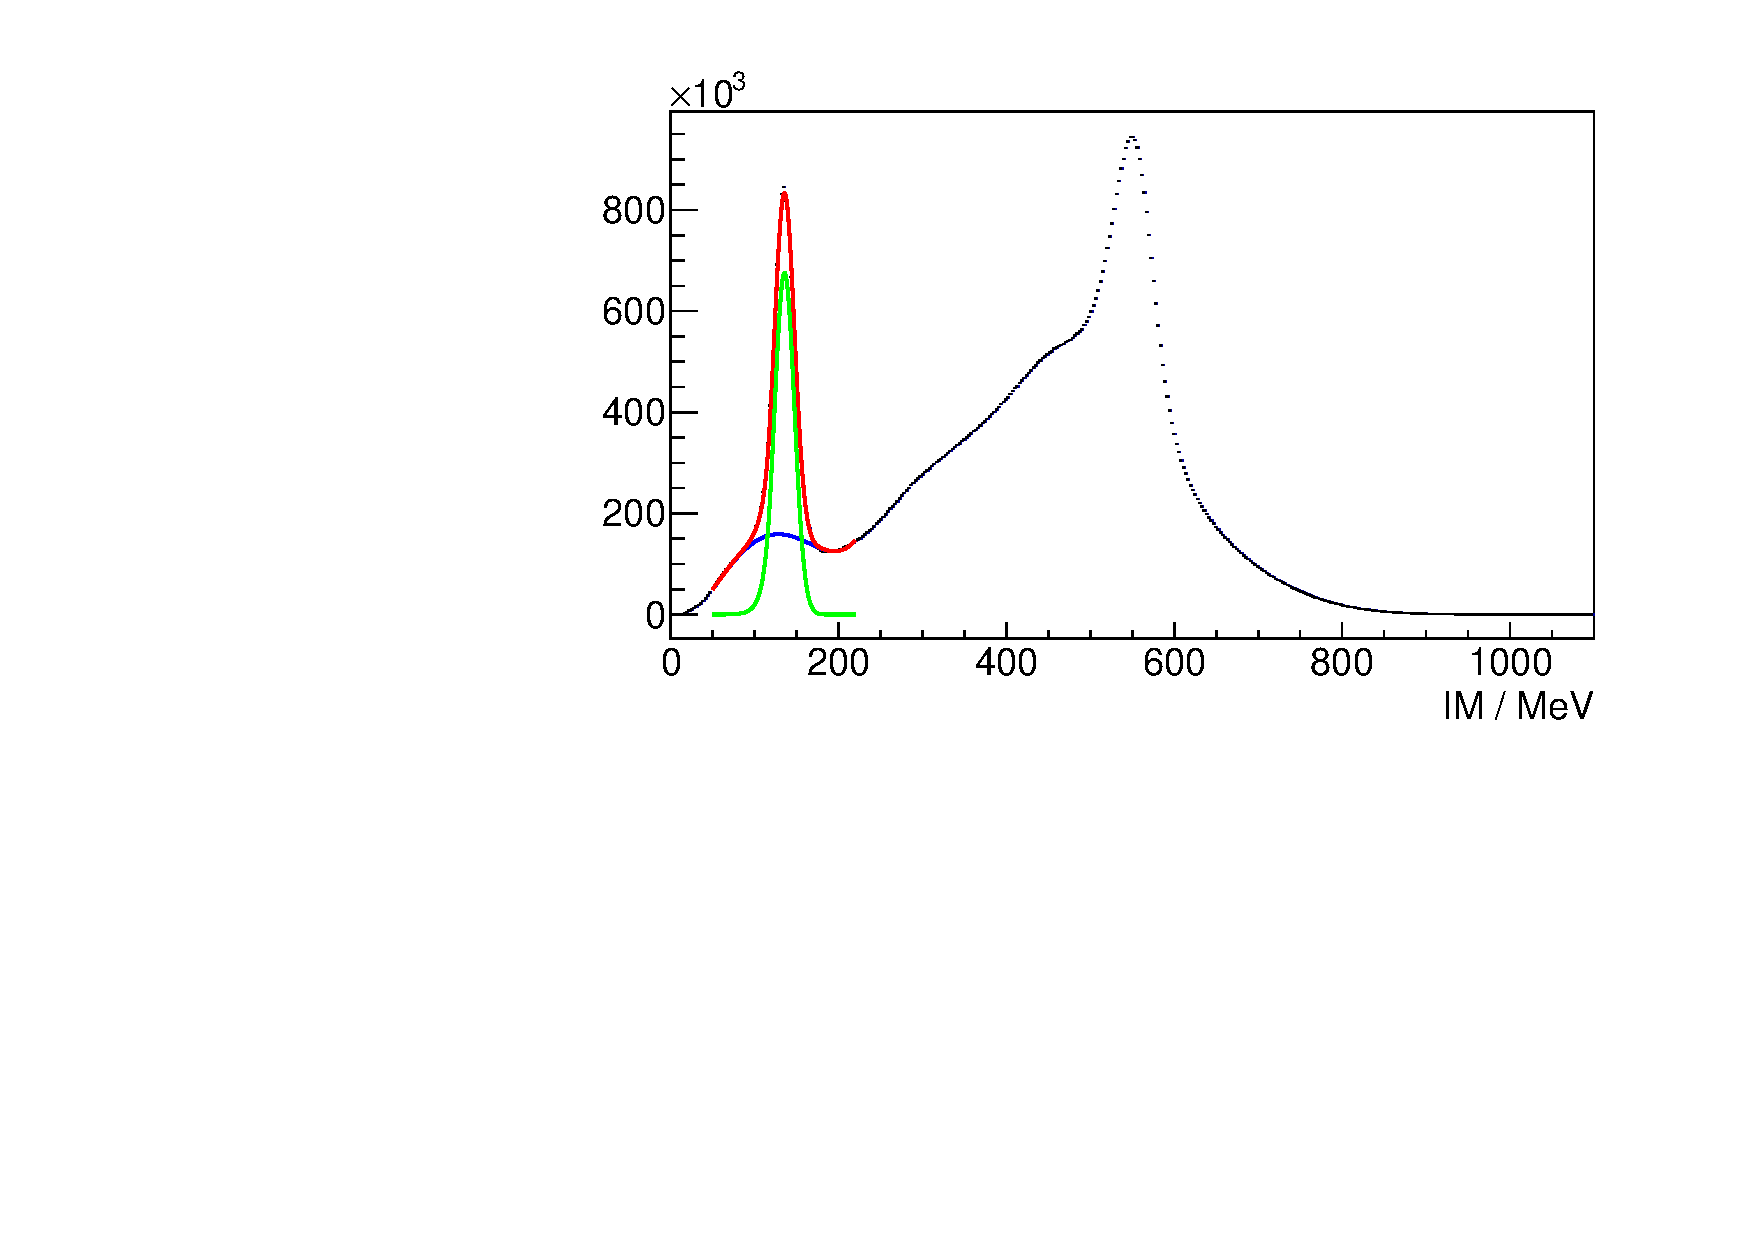
\includegraphics[width=0.50\textwidth]{Pictures/20171904RealIntervalFitExample}
	\hfill
		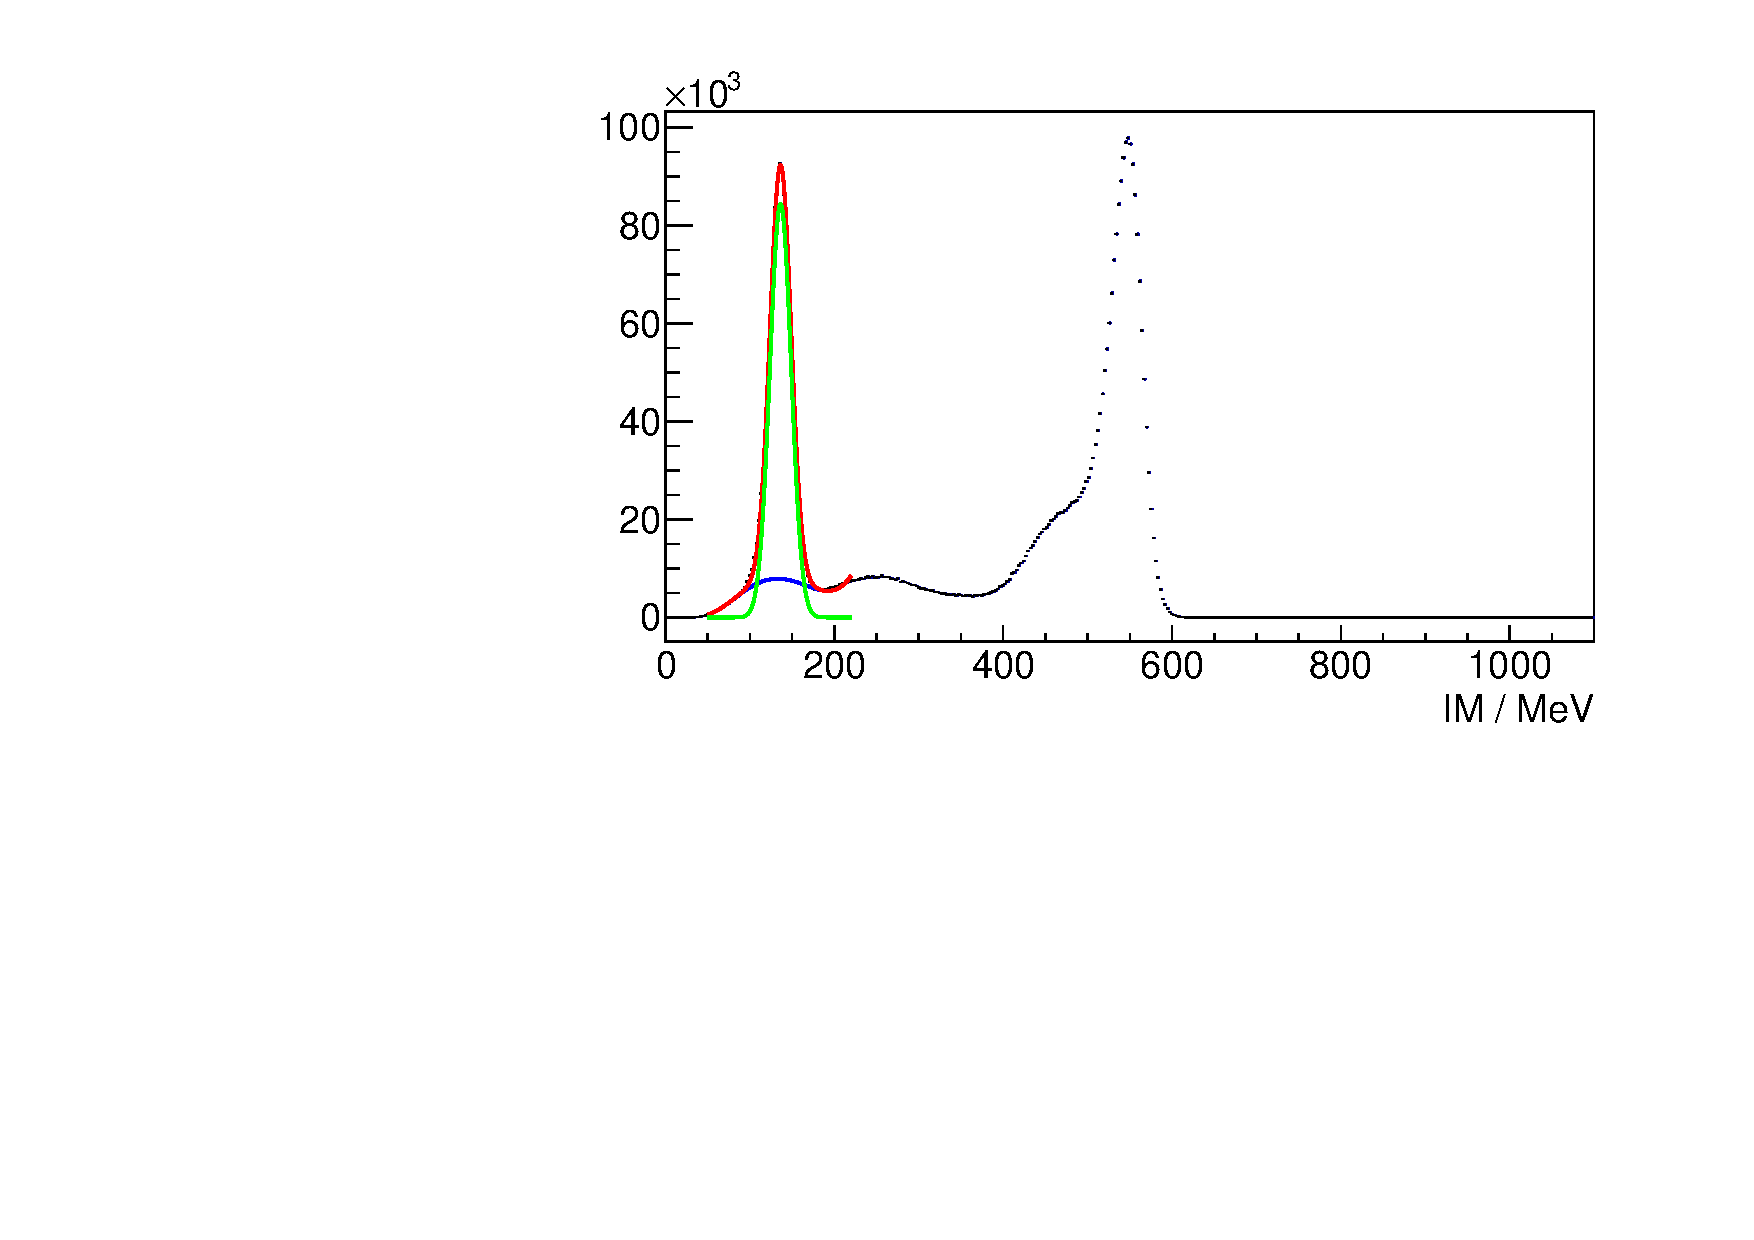
\includegraphics[width=0.50\textwidth]{Pictures/20171904RealUnchargedFitExample}
		\caption{Beamtime: Example for not reduced and reduced underground}
\end{figure}
\begin{tikzpicture}[remember picture,overlay]   
\coordinate (b) at (5.0 , 3.5);
\coordinate (c) at (5.7 , 3.5);
\draw [thick,black, ->,thick] (b) -- (c);
\end{tikzpicture}

\end{frame}
\begin{frame}
\frametitle{Event Generator}
Reasons for a new event generator:
\pause
\begin{itemize}
	\item The condition $|E_1 - E_2|<25\,\text{MeV}$ is a strong cut 
	
	$\rightarrow$ There is no package with enough events
	\pause
	
	\item Creating a new package with enough events would take to much time (multiple days on blaster)
	\pause
	
	\item It would be better if the same generator is used for all studies
	
	$\rightarrow$ The generator should be able to simulate MAMI-Beam and isotropic decay 
\end{itemize}
\end{frame}

\begin{frame}
	\frametitle{Event Generator}
\end{frame}
\section{Studies}


\begin{frame}
	\frametitle{No Additional Cut }
	
	\begin{itemize}
		\item Beamtime October 2014
		\item No additional cut
\end{itemize}
	
		\begin{figure}
		
		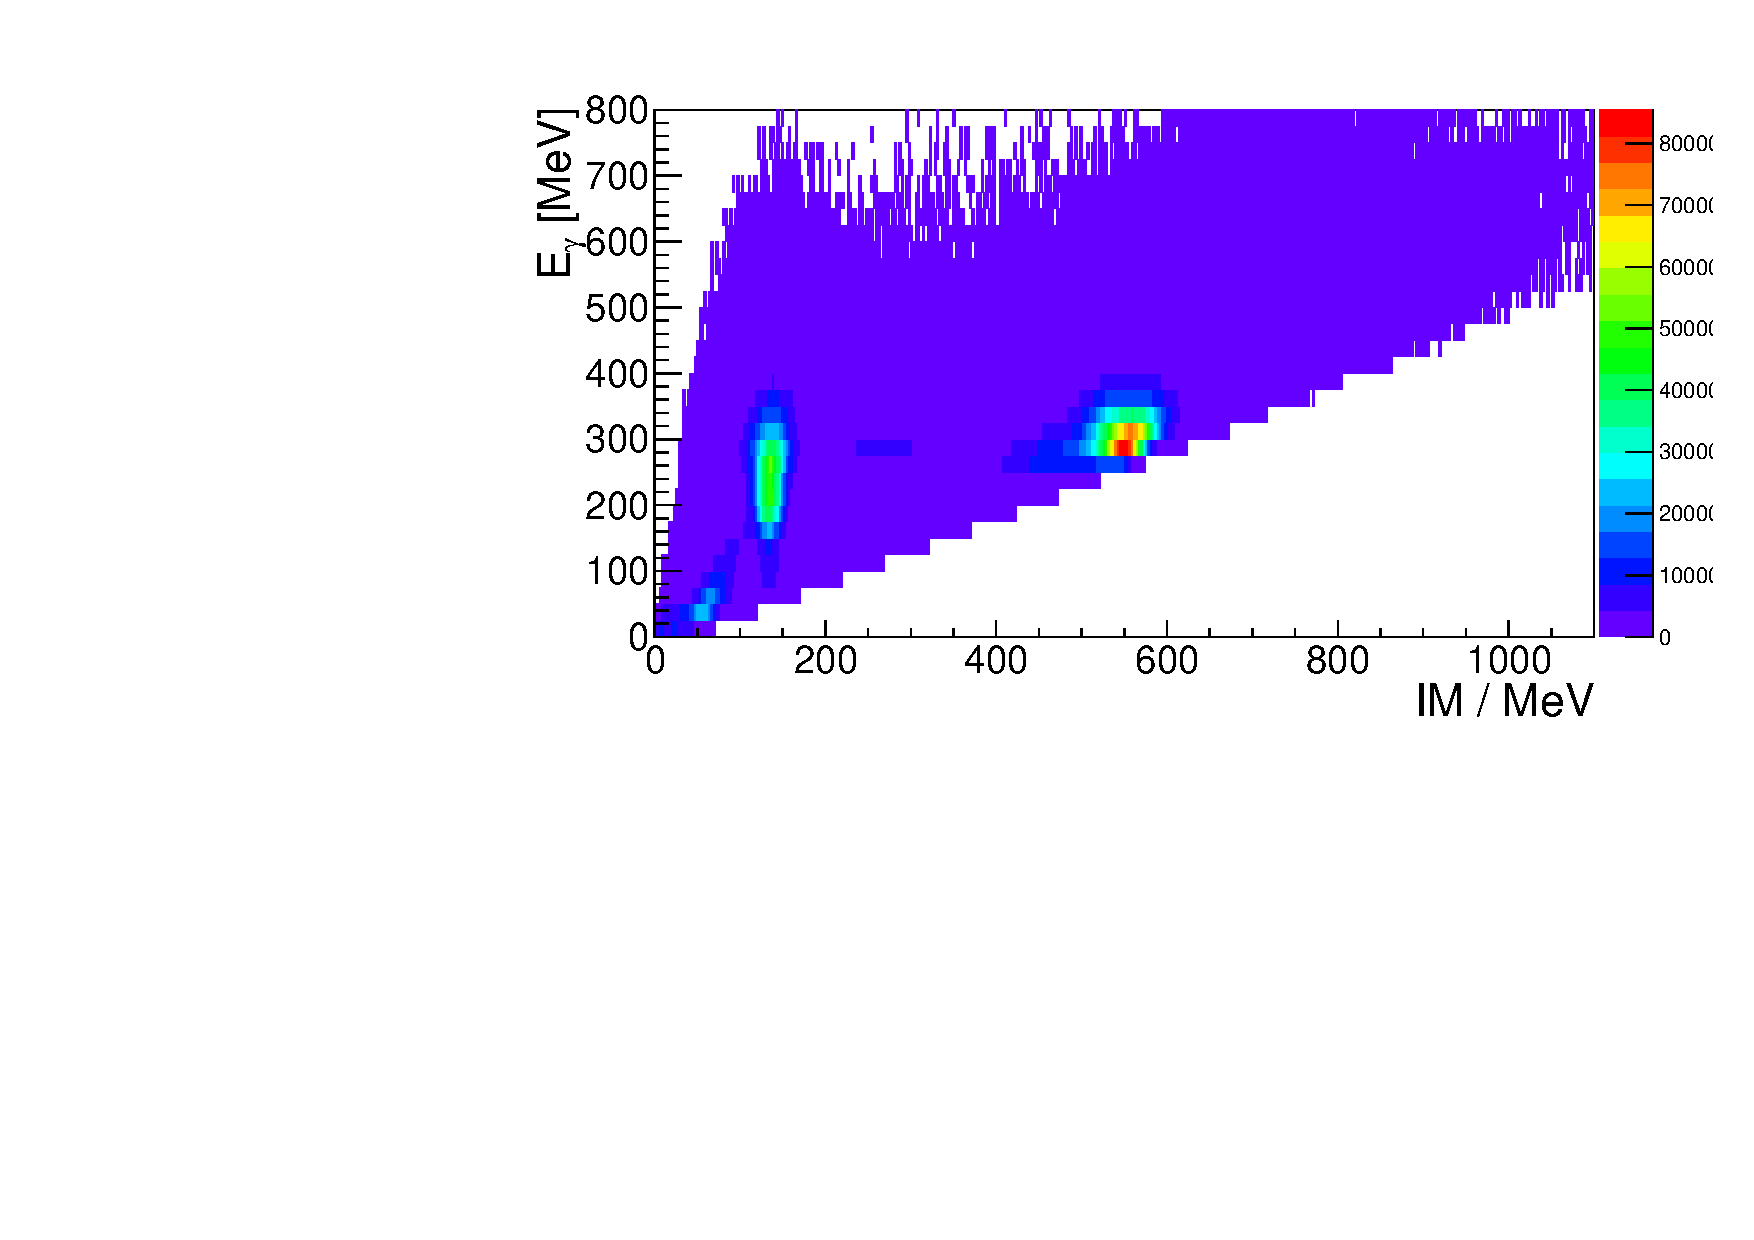
\includegraphics[width=0.50\textwidth]{Pictures/20171904Uncharged2DHist}
		\hfill
		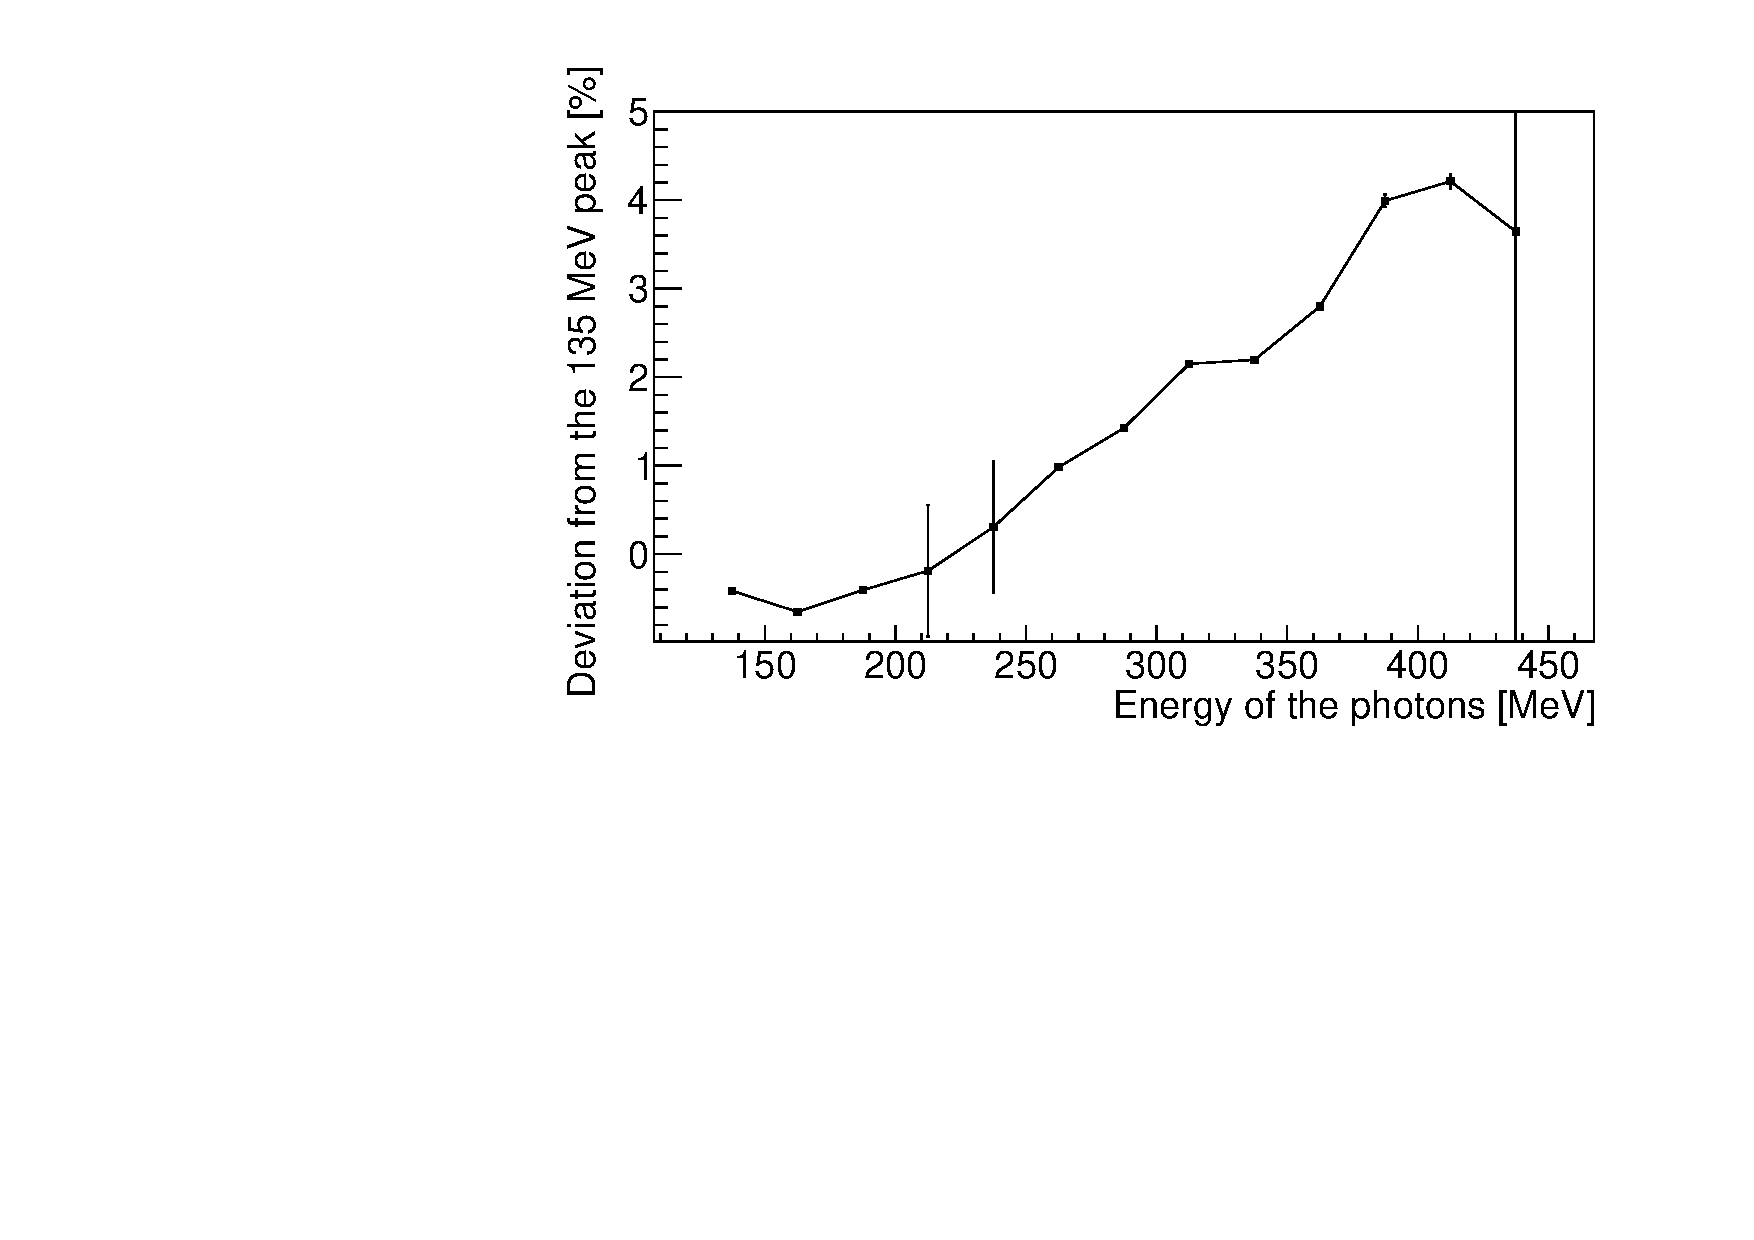
\includegraphics[width=0.50\textwidth]{Pictures/20170405StrahlzeitDeviatoinNoCut}
		\caption{Beamtime: No additional cut}
	\end{figure}	
\end{frame}

\begin{frame}
	\frametitle{Detectors On At The Edge}
	
	\begin{itemize}
		\item Beamtime October 2014
		\item Neglect the detectors at the edge
	\end{itemize}

\begin{figure}
	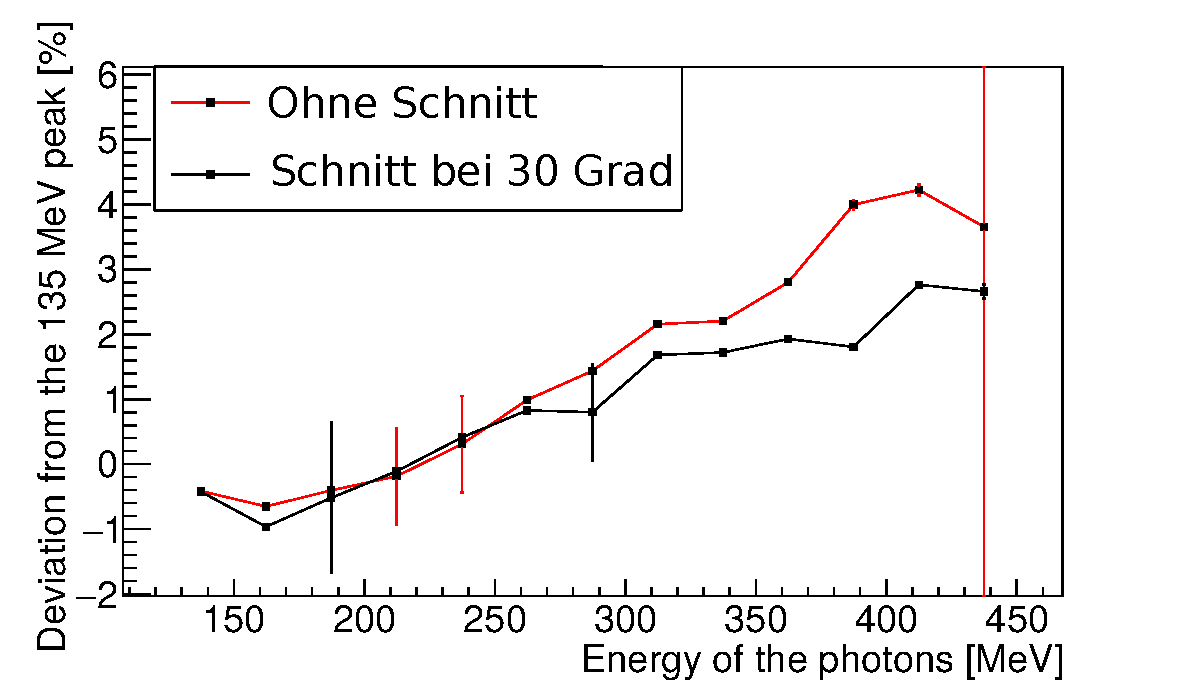
\includegraphics[width=0.75\textwidth]{Pictures/20170405StrahlzeitBothDeviation}
	\caption{Beamtime: With and without considerations of the detectors on the edge of the beam entrance and exit }
\end{figure}	
\end{frame}

\begin{frame}
	\frametitle{Simulation }
\end{frame}

\section{Further Results}
\begin{frame}
	\frametitle{Hot and Dead Crystals}
	
\end{frame}
\end{document} 